\documentclass[11pt,twocolumn]{article}
\usepackage{lmodern,setspace,amsmath,amssymb,amsfonts,amsthm,graphicx,multicol}
\usepackage[a4paper, top=0.9in, bottom=1.15in]{geometry}
\usepackage[polish]{babel}
\usepackage[utf8]{inputenc}
\title{Algorytmy i struktury danych - Programowanie dynamiczne}
\author{Dariusz Max Adamski}
\date{}

\begin{document}

\maketitle


\section*{Wstęp}

W tym sprawozdaniu będzie porównywana efektywność algorytmu zachłannego,
przeszukiwania wyczerpującego oraz algorytmu dynamicznego,
w rozwiązywaniu problemu plecakowego.
Skonfrontowane będą także algorytmy pod względem jakości uzyskanych rozwiązań.


\section*{Metodologia}

Optymalizacje kompilatora zostały wyłączone flagą ,,-O0''. 
Czas wykonywania był mierzony w nanosekundach.


\section{Efektywność algorytmów}

\begin{figure}[h!]
	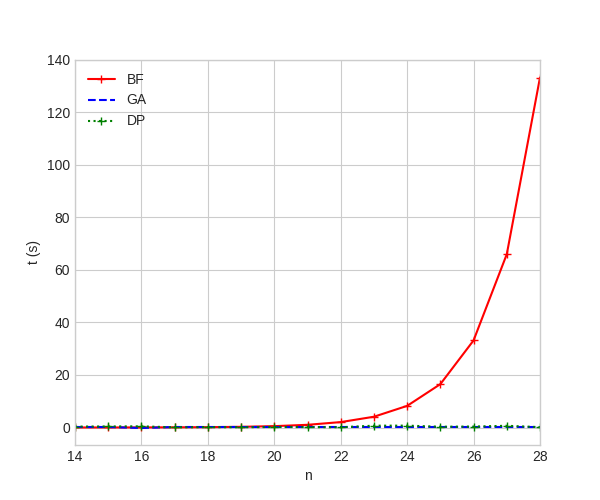
\includegraphics[width=\linewidth]{speed-n.png}
	\caption{Efektywność algorytmów w zależności od $n$ \label{speed_n}}
\end{figure}

Algorytm BF ma złożoność $O(2^n)$, co widać na wykresie \ref{speed_n}.
Krzywa BF może być aproksymowana przez funkcję
$BF'(n) = 2^n \cdot C = 2^{n + 20.6}$,
co potwierdza jej przynależność do klasy złożoności.

\begin{figure}[h!]
	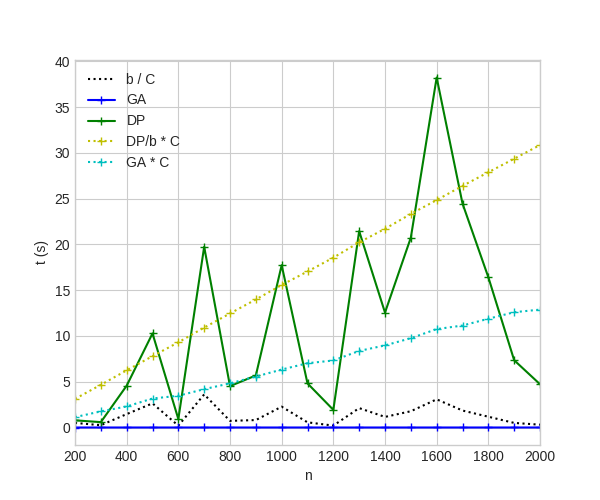
\includegraphics[width=\linewidth]{speed-n-big.png}
	\caption{Efektywność algorytmów w zależności od $n$ \label{speed_n_big}}
\end{figure}

Czasy wykonywania GA oraz DP dla $n > 28$, są przedstawione na wykresie \ref{speed_n_big}.
Złożoność GA to $O(n \log n)$. Rzeczywisty czas wykonywania jest oznaczony jako GA.
Funkcja została także przeskalowana o stałą $C$ i przedstawiona na wykresie jako ,,GA * C'',
aby lepiej zilustrować czas wykonywania.

Analiza złożoności DP jest trudniejsza, 
ponieważ zależy ona od dwóch zmiennych $b$ oraz $n$.
Na wykresie \ref{speed_n_big} jest przedstawiona funkcja $DP/b$,
przeskalowana o stałą $C$ która pokazuje, że 
DP rośnie liniowo w zależności od $n$.
Ewentualne odchylenia są spowodowane losowością instancji problemu.

Aby mieć pewność, że $b$ nie jest zależne od $n$, na rysunku została
pokazana relacja $b$ od $n$, przeskalowana o stałą $C$.
Jak widać, jest ona losowa.
Możemy więc potwierdzić, że złożoność DP to faktycznie $O(b \cdot n)$.

\begin{figure}[h!]
	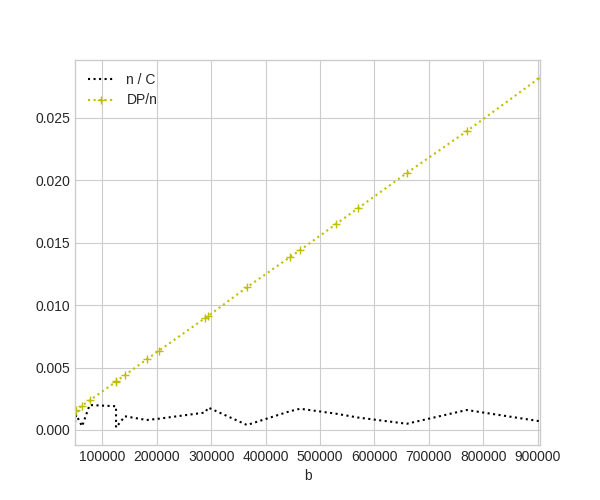
\includegraphics[width=\linewidth]{speed-b-big.png}
	\caption{Efektywność algorytmów w zależności od $b$ \label{speed_b_big}}
\end{figure}

Następnie na wykresie \ref{speed_b_big} została przedstawiona zależność ,,DP/n'' 
Jak widać DP rośnie także liniowo w zależności od $b$.
Dodatkowo na wykresie znajduje się relacja $n$ od $b$, przeskalowana o stałą $C$.

\begin{figure}[h!]
	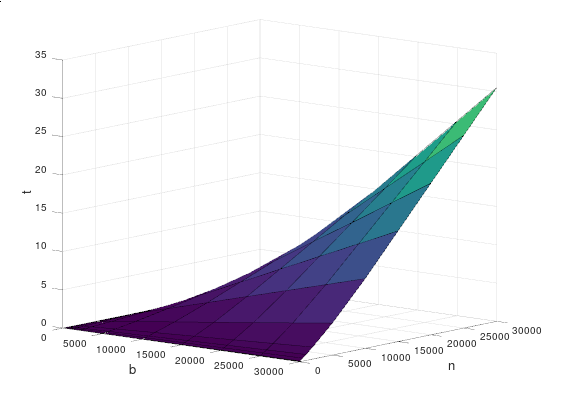
\includegraphics[width=\linewidth]{speed-bn.png}
	\caption{Efektywność DP w zależności od $n$ i $b$ \label{speed_bn}}
\end{figure}

\section{Jakość rozwiązań}

\section{Podsumowanie}

Problem plecakowy jest problemem należącym do części wspólnej klas NP oraz NP-hard, czyli NP-complete, zakładając że $P \neq NP$.

\begin{figure}[h!]
	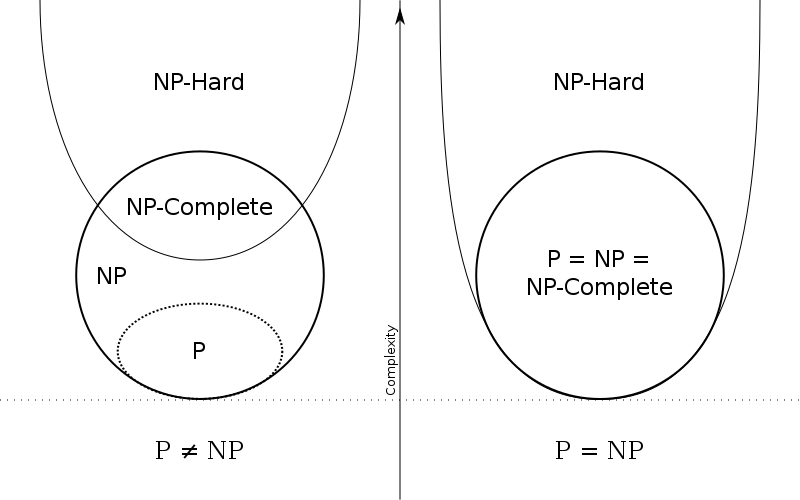
\includegraphics[width=\linewidth]{pnp.png}
\end{figure}

Oznacza to operacja znajdywania rozwiązania problemu ma złożoność najwyżej wykładniczą.
Możemy jednak zweryfikować znalezione rozwiązanie w czasie wielomianowym.

Podsumowując, metodą najlepiej rozwiązującą problem plecakowy
jest programowanie dynamiczne. Ta metoda działa zdecydowanie szybciej od
przeszukiwania wyczerpującego i w odróżnieniu od algorytmu zachłannego
nie aproksymuje rozwiązania.
Jednak jeżeli możemy pozwolić sobie na aproksymację rozwiązania,
algorytm zachłanny zapewnia je w czasie wielomianowym.

\end{document}
